% Copyright 2026 Sreeram Anil
% SPDX-License-Identifier: CC-BY-4.0
% =============================================================================
%  TRIAD — single-frame attitude determination, attitude (AHRS) family
% =============================================================================
\chapter{Single-Frame Attitude Determination: TRIAD}
\label{ch:att-triad}

\section*{At a glance}
\begin{tabular}{@{}l>{\raggedright\arraybackslash}p{0.76\textwidth}@{}}
Family & attitude / AHRS (memory-less baseline) \\
Header & \texttt{include/estkit/attitude/triad\_quest.hpp} \\
Registered name & \texttt{TRIAD} \\
State & none: $\bm{q}_k$ is a function of $(\bm{f}_k,\bm{m}_k)$ alone \\
Cost per step & $\approx120$ flops, one \code{sqrt};
  $\SI{129}{\nano\second}$/step, 120\,bytes \\
Primary references & \cite{black1964,shusteroh1981,markleymortari2000} \\
\end{tabular}

\section{Motivation and aerospace relevance}
Every estimator in this family except this one and its sibling (Chapter~\ref{ch:att-quest}) carries
state. TRIAD carries none: it solves for the attitude from the two vector observations available at
the current instant and throws the answer away. Black's 1964 note~\cite{black1964} --- two pages,
written for the Transit navigation satellites --- is the oldest attitude algorithm still in routine
use, and it is the one an AHRS falls back to for coarse alignment, for sanity-checking a filter, and
for initialising one.

Its role in this benchmark is diagnostic. Because it has no memory, no tuning and no dynamics
model, its error \emph{is} the instantaneous inconsistency of the sensor pair: it measures the
quality of the measurements, not the quality of an algorithm. Every filtered estimator in the family
should be read against it --- what a filter achieves \emph{below} the TRIAD error is exactly what
its memory bought, and where a filter is no better than TRIAD, its memory is not being used.

\section{Problem statement and assumptions}
Given $m=2$ pairs of unit vectors, $\bm{b}_i$ in the BODY frame and $\bm{r}_i$ in the NAV frame,
related by an unknown rotation,
\begin{equation}
\bm{b}_i \;=\; \bm{R}^\T\bm{r}_i + \text{noise},\qquad i=1,2,
\label{eq:tr-obs}
\end{equation}
find $\bm{R}\in SO(3)$. Here $\bm{r}_1=[0,0,-1]^\T$ with $\bm{b}_1=\bm{f}/\norm{\bm{f}}$ (the NED
reference of a normalised specific-force measurement) and
$\bm{r}_2=\bm{m}_{\text{nav}}/\norm{\bm{m}_{\text{nav}}}$ with $\bm{b}_2=\bm{m}/\norm{\bm{m}}$.

Two observations are the minimum: one unit vector fixes two degrees of freedom and leaves the
rotation about itself free. Two are also, in general, one too many --- \eqref{eq:tr-obs} is
over-determined (four independent constraints for three unknowns) and generally inconsistent, since
the measured angle between $\bm{b}_1$ and $\bm{b}_2$ will not equal the reference angle between
$\bm{r}_1$ and $\bm{r}_2$. TRIAD resolves the inconsistency by fiat: it satisfies one observation
\emph{exactly} and uses the other only for the remaining degree of freedom. Which one is
``primary'' is the method's only design choice.

\section{Derivation}
Let $\bm{b}_p,\bm{r}_p$ be the primary pair and $\bm{b}_s,\bm{r}_s$ the secondary pair. Build two
right-handed orthonormal triads, one from the body observations and one from the references:
\begin{equation}
\bm{t}_1 = \bm{b}_p,\quad
\bm{t}_2 = \frac{\bm{b}_p\times\bm{b}_s}{\norm{\bm{b}_p\times\bm{b}_s}},\quad
\bm{t}_3 = \bm{t}_1\times\bm{t}_2;
\qquad
\bm{u}_1 = \bm{r}_p,\quad
\bm{u}_2 = \frac{\bm{r}_p\times\bm{r}_s}{\norm{\bm{r}_p\times\bm{r}_s}},\quad
\bm{u}_3 = \bm{u}_1\times\bm{u}_2 .
\label{eq:tr-triads}
\end{equation}
Both $[\bm{t}_1\,\bm{t}_2\,\bm{t}_3]$ and $[\bm{u}_1\,\bm{u}_2\,\bm{u}_3]$ are orthogonal matrices
by construction, so
\begin{equation}
\bm{R} \;=\; [\bm{u}_1\,\bm{u}_2\,\bm{u}_3]\,[\bm{t}_1\,\bm{t}_2\,\bm{t}_3]^\T
 \;=\; \sum_{i=1}^{3}\bm{u}_i\bm{t}_i^\T \;\in\;SO(3)
\label{eq:tr-R}
\end{equation}
is a rotation, and $\bm{R}\bm{b}_p=\bm{u}_1=\bm{r}_p$ exactly: the primary observation is satisfied
without residual, while the secondary contributes only through the plane it spans with the primary
(its component along $\bm{b}_p$ is discarded). \eqref{eq:tr-R} needs no iteration, no
decomposition, and no trigonometry.

The rotation matrix is converted to a quaternion by Shepperd's algorithm~\cite{shepperd1978}, which
selects the largest of $\{\tr\bm{R},R_{11},R_{22},R_{33}\}$ so that the divisor is never below
$\tfrac12$ and the relative error is bounded for any rotation, including the $180^\circ$ case where
the naive trace formula loses all precision. The mission yaw passes through $\pm180^\circ$ twice, so
this is not a hypothetical.

\subsection{Error behaviour and the degeneracy}
Perturb the secondary observation by an angle $\varepsilon_s$. Its component perpendicular to
$\bm{b}_p$ is what determines $\bm{t}_2$, so the resulting attitude error about $\bm{b}_p$ is
\begin{equation}
\delta\vartheta \;\approx\; \frac{\varepsilon_s}{\sin\gamma},
\qquad \gamma = \angle(\bm{b}_p,\bm{b}_s),
\label{eq:tr-amplify}
\end{equation}
while a perturbation $\varepsilon_p$ of the primary passes through unattenuated. Two consequences:
\begin{itemize}[nosep]
\item TRIAD is \emph{asymmetric}. All of the primary sensor's error enters the answer; only the
perpendicular part of the secondary's does, amplified by $1/\sin\gamma$. Shuster and
Oh~\cite{shusteroh1981} show that TRIAD is the limit of the optimal weighted solution
(Chapter~\ref{ch:att-quest}) as the primary weight tends to infinity, which makes it optimal only if
the primary sensor really is much better than the secondary.
\item TRIAD is \emph{ill-conditioned when the observations are nearly collinear or
anti-collinear}. At $\gamma\to0$ or $\pi$ the cross product in \eqref{eq:tr-triads} vanishes and
$\bm{t}_2$ is defined by noise alone. This is not an academic concern in an AHRS at high magnetic
latitude: see the results.
\end{itemize}

\section{Algorithm}
\begin{algorithm}[H]
\caption{TRIAD --- one sampling period (the gyroscope is ignored)}
\begin{algorithmic}[1]
\Require $\bm{f},\bm{m}$; references $\bm{r}_1=[0,0,-1]^\T$, $\bm{r}_2=\hat{\bm{m}}_{\text{nav}}$
\State \textbf{if} $\norm{\bm{f}}$ or $\norm{\bm{m}}$ is negligible \textbf{then return} previous $\bm{q}$
\State $\bm{b}_1\gets\bm{f}/\norm{\bm{f}}$;\; $\bm{b}_2\gets\bm{m}/\norm{\bm{m}}$
\State $(\bm{b}_p,\bm{r}_p,\bm{b}_s,\bm{r}_s)\gets$ primary/secondary assignment
\State $\bm{t}_2\gets\widehat{\bm{b}_p\times\bm{b}_s}$;\; $\bm{t}_3\gets\bm{b}_p\times\bm{t}_2$;\;
       $\bm{u}_2\gets\widehat{\bm{r}_p\times\bm{r}_s}$;\; $\bm{u}_3\gets\bm{r}_p\times\bm{u}_2$
\State $\bm{R}\gets\bm{r}_p\bm{b}_p^\T+\bm{u}_2\bm{t}_2^\T+\bm{u}_3\bm{t}_3^\T$ \Comment{\eqref{eq:tr-R}}
\State $\bm{q}_k\gets\text{Shepperd}(\bm{R})$, normalise
\Ensure $\bm{q}_k$
\end{algorithmic}
\end{algorithm}

\section{Application to the benchmark flight}
The registered configuration takes the accelerometer as primary (\code{primary = 0}), which is the
usual AHRS choice: the specific force has twice the direction accuracy of the
magnetometer in the absence of manoeuvres ($\sigma_a/g=\SI{5.1e-3}{\radian}$ against
$\sigma_m/B=\SI{10.4e-3}{\radian}$ on the nominal scenario) and the magnetometer is the sensor with
the systematic error (hard iron). There is nothing else to configure: no gains, no covariance, no
initial condition --- \code{reset()} stores $\bm{q}_0$ only so that \code{quaternion()} is defined
before the first sample.

\section{Implementation notes}
Two cross products, two normalisations, three outer products (27 multiply--adds) and one Shepperd
conversion: about 120 flops, one \code{sqrt} beyond the two measurement normalisations. Measured
$\SI{129}{\nano\second}$/step and 120\,bytes, the smallest state of any estimator in the family and
within $\SI{20}{\nano\second}$ of the fastest. On a Cortex-M4 without an FPU this is a few
microseconds, which is why it is the universal power-on alignment routine.

Numerical hygiene: \code{att::unit()} returns its argument unchanged rather than dividing by zero
when the norm is below $10^{-12}$, so a vanishing cross product degrades to a non-orthogonal
$\bm{R}$ rather than to NaN; the step is skipped entirely if either measurement magnitude is below
$10^{-6}$, leaving the previous quaternion in place; Shepperd's branch selection bounds the
conversion error. No NaN or infinity was produced on any of the six scenarios
($1.6\times10^{6}$ samples over three seeds). The single-precision build reproduces the
double-precision mission RMS to four digits.

The structural limitation needs no analysis: with no state, the estimate cannot be better than the
worse of the two instantaneous measurements, and the \emph{time} axis --- which contains all the
information the gyroscope provides --- is unused.

\section{Benchmark results}
% Copyright 2026 Sreeram Anil
% SPDX-License-Identifier: CC-BY-4.0
\begin{table}[H]\centering\footnotesize\setlength{\tabcolsep}{3.5pt}\caption{TRIAD: attitude benchmark (mean over seeds; all angles in degrees; $t_\mathrm{conv}$: first time the attitude error stays below 2$^\circ$ for 30\,s; bias RMSE in deg/s; 120 bytes of state).}\label{tab:imu_TRIAD}
\begin{tabular}{lrrrrrrrrcr}\toprule scenario & RMS & roll & pitch & yaw & max & RMS$_\mathrm{ss}$ & $t_\mathrm{conv}$ [s] & bias RMSE & lost & ns/step \\ \midrule
nominal & 19.59 & 9.37 & 1.45 & 17.17 & 88.2 & 21.60 & -- & 1.03 & yes & 129 \\
init\_error & 19.59 & 9.37 & 1.45 & 17.17 & 88.2 & 21.60 & -- & 1.03 & yes & 129 \\
gyro\_bias & 19.59 & 9.37 & 1.45 & 17.17 & 88.2 & 21.60 & -- & 3.80 & yes & 129 \\
mag\_disturbance & 20.97 & 9.37 & 1.45 & 18.73 & 88.2 & 21.60 & -- & 1.03 & yes & 129 \\
vibration & 27.26 & 11.20 & 6.23 & 24.25 & 179.7 & 29.35 & -- & 1.03 & yes & 129 \\
high\_dynamics & 20.98 & 9.80 & 1.59 & 18.57 & 139.0 & 23.00 & -- & 1.03 & yes & 128 \\
\bottomrule\end{tabular}\end{table}

\begin{figure}[H]\centering
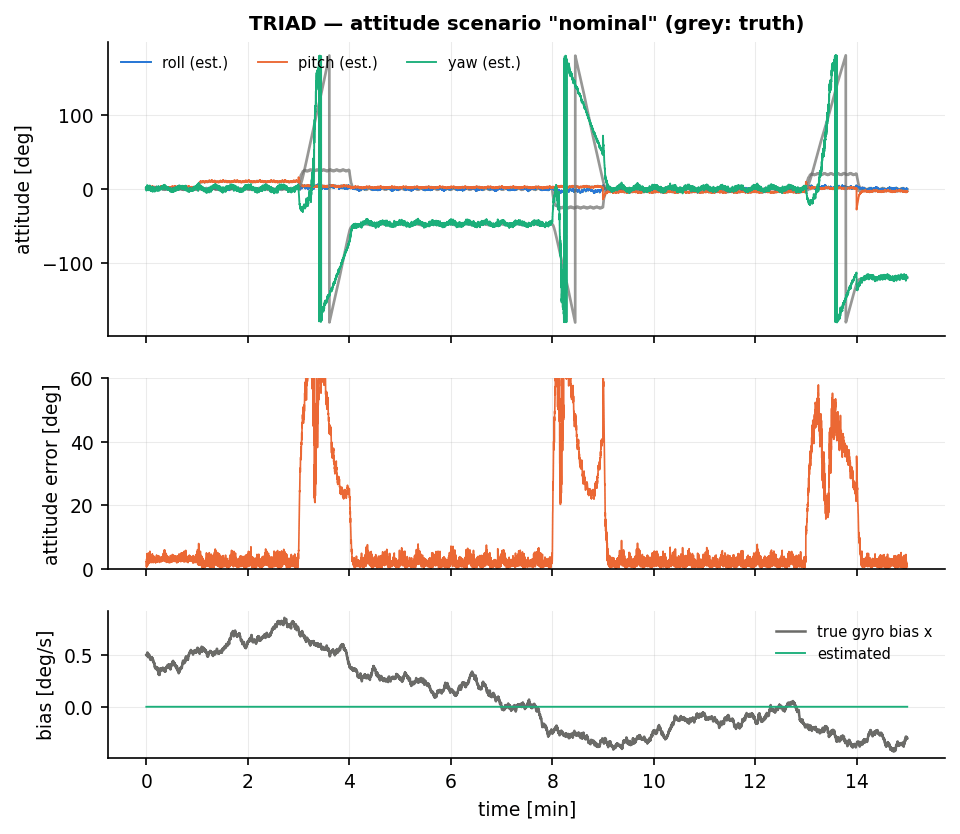
\includegraphics[width=\textwidth]{figures/imu_TRIAD_nominal.png}
\caption{TRIAD on the nominal mission. The three coordinated turns are visible as
$\SI{45}{\degree}$ error plateaus; between them the estimate tracks truth to a few degrees with no
filtering at all.}
\end{figure}
\begin{figure}[H]\centering
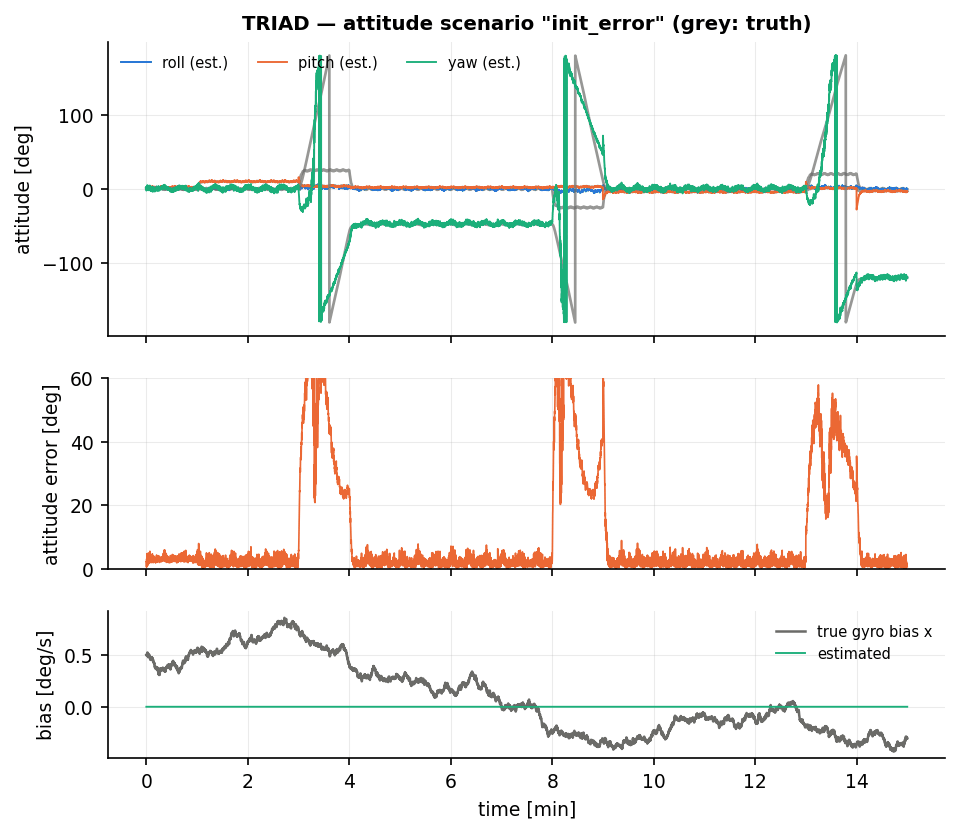
\includegraphics[width=\textwidth]{figures/imu_TRIAD_init_error.png}
\caption{TRIAD with a $46.6^\circ$ initial error --- which it does not see, being memory-less: the
trace is identical to the nominal one.}
\end{figure}

\paragraph{Insensitivity to initialisation and to the gyroscope.} \texttt{nominal},
\texttt{init\_error} and \texttt{gyro\_bias} give \emph{identical} results,
$\text{RMS}=\SI{19.59}{\degree}$, because the estimate depends on neither the initial condition nor
the gyroscope. Starting from $90^\circ$ of attitude error, TRIAD is inside $5^\circ$ at the first
sample. That is the memory-less method's one genuine advantage, and it is the reason every
practical AHRS uses it for coarse alignment: it cannot be wrong for longer than one sample because
of something that happened earlier. (Its \emph{bias} RMSE column simply reports the true bias
magnitude, $1.03$ and $\SI{3.80}{\degree\per\second}$, since it estimates none.)

\paragraph{Accelerated flight: the quantification.} Per phase on \texttt{nominal} (seed~1),
\[
3.13\;/\;2.59\;/\;\mathbf{45.21}\;/\;2.55\;/\;\mathbf{43.30}\;/\;2.51\;/\;\mathbf{36.40}\;/\;2.08
\ \SI{}{\degree}
\]
for take-off / climb / turn\,1 / cruise / turn\,2 / descent / turn\,3 / final; mission RMS
$\SI{19.59}{\degree}$, $\text{RMS}_{\text{ss}}=\SI{21.60}{\degree}$, peak $\SI{88.2}{\degree}$. In
unaccelerated flight TRIAD is a $\SI{2.5}{\degree}$--$\SI{3.1}{\degree}$ device --- within
$\SI{1.5}{\degree}$ of the six-state MEKF in the same phases
($1.30/1.50/1.74/1.91/\SI{1.86}{\degree}$), at $1/16$ of the cost --- and during the three
$\SI{60}{\second}$ coordinated turns it is a $\SI{36}{\degree}$--$\SI{45}{\degree}$ device. The
mechanism has two stages, and both are amplifications:
\begin{enumerate}[nosep]
\item In a coordinated turn the specific force lies along the body $z$ axis, so the primary
observation is wrong by the full bank angle, $\approx25^\circ$ at $t=\SI{488}{\second}$ (measured:
$\bm{f}=[-0.55,-0.81,-10.20]^\T$ against a true bank of $-24.75^\circ$). TRIAD satisfies the primary
\emph{exactly}, so this error enters the answer undiminished.
\item The magnetic field at $I=65^\circ$ has a vertical component of $\SI{43.5}{\micro\tesla}$
against $\SI{20.3}{\micro\tesla}$ horizontal. A tilt error therefore leaks into the heading with
gain $\tan I=2.14$: the $25^\circ$ tilt error becomes $\approx50^\circ$ of heading error, which is
why the yaw RMS ($\SI{17.17}{\degree}$) is nearly twice the roll RMS ($\SI{9.37}{\degree}$).
\end{enumerate}
Note that recalibrating the compass (the dataset's residual hard iron is now
$\SI{0.42}{\micro\tesla}$, a $\SI{0.65}{\degree}$ heading floor) improved the level-flight phases by
about $\SI{1.4}{\degree}$ but left the mission RMS essentially unchanged: the turns dominate, and
they are an accelerometer problem, not a magnetometer problem.

\paragraph{The collinearity degeneracy.} On \texttt{vibration} the mission RMS rises to
$\SI{27.26}{\degree}$ and the peak reaches $179.7^\circ$; $986$ of the $9\times10^4$ samples
($1.1\,\%$) exceed $90^\circ$ of error. This is \eqref{eq:tr-amplify} firing. At
$t=\SI{488.17}{\second}$ --- inside the second turn, at $-24.75^\circ$ of bank --- the measured
directions are $\bm{f}=[-0.55,-0.81,-10.20]^\T$ and $\bm{m}=[2.05,0.51,47.69]^\T$, i.e.
$\gamma=176.1^\circ$ apart, so $\norm{\bm{b}_1\times\bm{b}_2}=0.069$ and the amplification in
\eqref{eq:tr-amplify} is $1/0.069=14.5$. The reference pair is $155^\circ$ apart, so the
observations are also grossly inconsistent, and the triad construction returns an essentially
arbitrary rotation about $\bm{b}_1$. This is the practical meaning of the observability condition
$\bm{M}\succ0$ of Chapter~\ref{ch:att-mahony}, \eqref{eq:mh-lin}: two-vector attitude determination
degrades as $1/\sin\gamma$, and a steep turn at high magnetic dip drives $\gamma$ towards $\pi$.

\paragraph{The primary-sensor choice.} Making the \emph{magnetometer} primary improves the mission
RMS from $19.59$ to $\SI{18.52}{\degree}$ and the vibration case from $27.20$ to
$\SI{25.83}{\degree}$, and it redistributes the error (roll $9.37\to6.67$, pitch
$1.45\to\SI{3.74}{\degree}$). On this mission the magnetometer --- now well calibrated --- is the
more trustworthy of the two sensors, because the accelerometer is wrong by $25^\circ$ for a fifth of
the flight. That the ``obvious'' choice is the wrong one is the strongest argument for the weighted
solution of the next chapter, which does not have to choose at all.

\paragraph{Other scenarios.} \texttt{mag\_disturbance} costs $\SI{1.4}{\degree}$ ($20.97$): the
$\SI{25}{\micro\tesla}$ anomaly enters the secondary observation, attenuated by $1/\sin\gamma$,
and there is no mechanism to reject it. \texttt{high\_dynamics} costs $\SI{1.4}{\degree}$ ($20.98$,
peak $139^\circ$). The convergence metric is $-1$ and the \texttt{lost} flag is set on every
scenario --- the harness's $45^\circ$ threshold is exceeded in every turn by construction, which is
a correct description of the estimator, not a numerical failure.

\section{Summary}
TRIAD is two cross products and an orthogonalisation, 120\,bytes,
$\SI{0.13}{\micro\second}$/step, no tuning, and an answer that is independent of everything that
happened before the current sample. Use it for coarse alignment, for initialising a filter, and as
the honest lower bound on what instantaneous sensor data can deliver: in unaccelerated flight it
comes within $\SI{1.5}{\degree}$ of a six-state Kalman filter. Do not use it as an AHRS on a manoeuvring vehicle --- it satisfies the
accelerometer exactly, which is the worst possible policy when the accelerometer is the disturbed
sensor --- and be aware that its conditioning degrades as $1/\sin\gamma$ with the angle between the
two observations, which at $65^\circ$ of magnetic dip and $25^\circ$ of bank reaches
$\gamma=176^\circ$ --- close enough to $\pi$ to produce $180^\circ$ outliers in $1\,\%$ of the
samples of the \texttt{vibration} run.
